\documentclass{article}

\usepackage[T1]{fontenc}    %Schriftart des Dokumentes
\usepackage[ngerman]{babel} %Dokumentensprache, hier Deutsch
\usepackage{amsmath, amssymb, stmaryrd} %mathematische Schriftzeichen
\usepackage{graphicx} %Einfügen von Grafiken
\usepackage{wrapfig}
\usepackage{bm}
\usepackage{subfig}
\usepackage{newclude}
\usepackage{pdfpages}

\setlength{\parindent}{0pt} %Einrückung von Absätzen auf null gesetzt
\setlength{\parskip}{10pt} %Abstand zischen Absätzen auf 10pt gesetzt

\title{Versuch X: }
\author{Matthias Kuntz}
\date{date}

\renewcommand*\contentsname{Zusammenfassung}

\begin{document}

\maketitle

\tableofcontents

\newpage

%-------------------------EINLEITUNG-------------------------
\section{Einleitung}

\subsection{Physikalische Grundlagen}

\subsection{Versuchsaufbau}

%---------------VERSUCHSPROTOKOLL MIT MESSDATEN---------------
\newpage

\section{Versuchsprotokoll mit Messdaten}

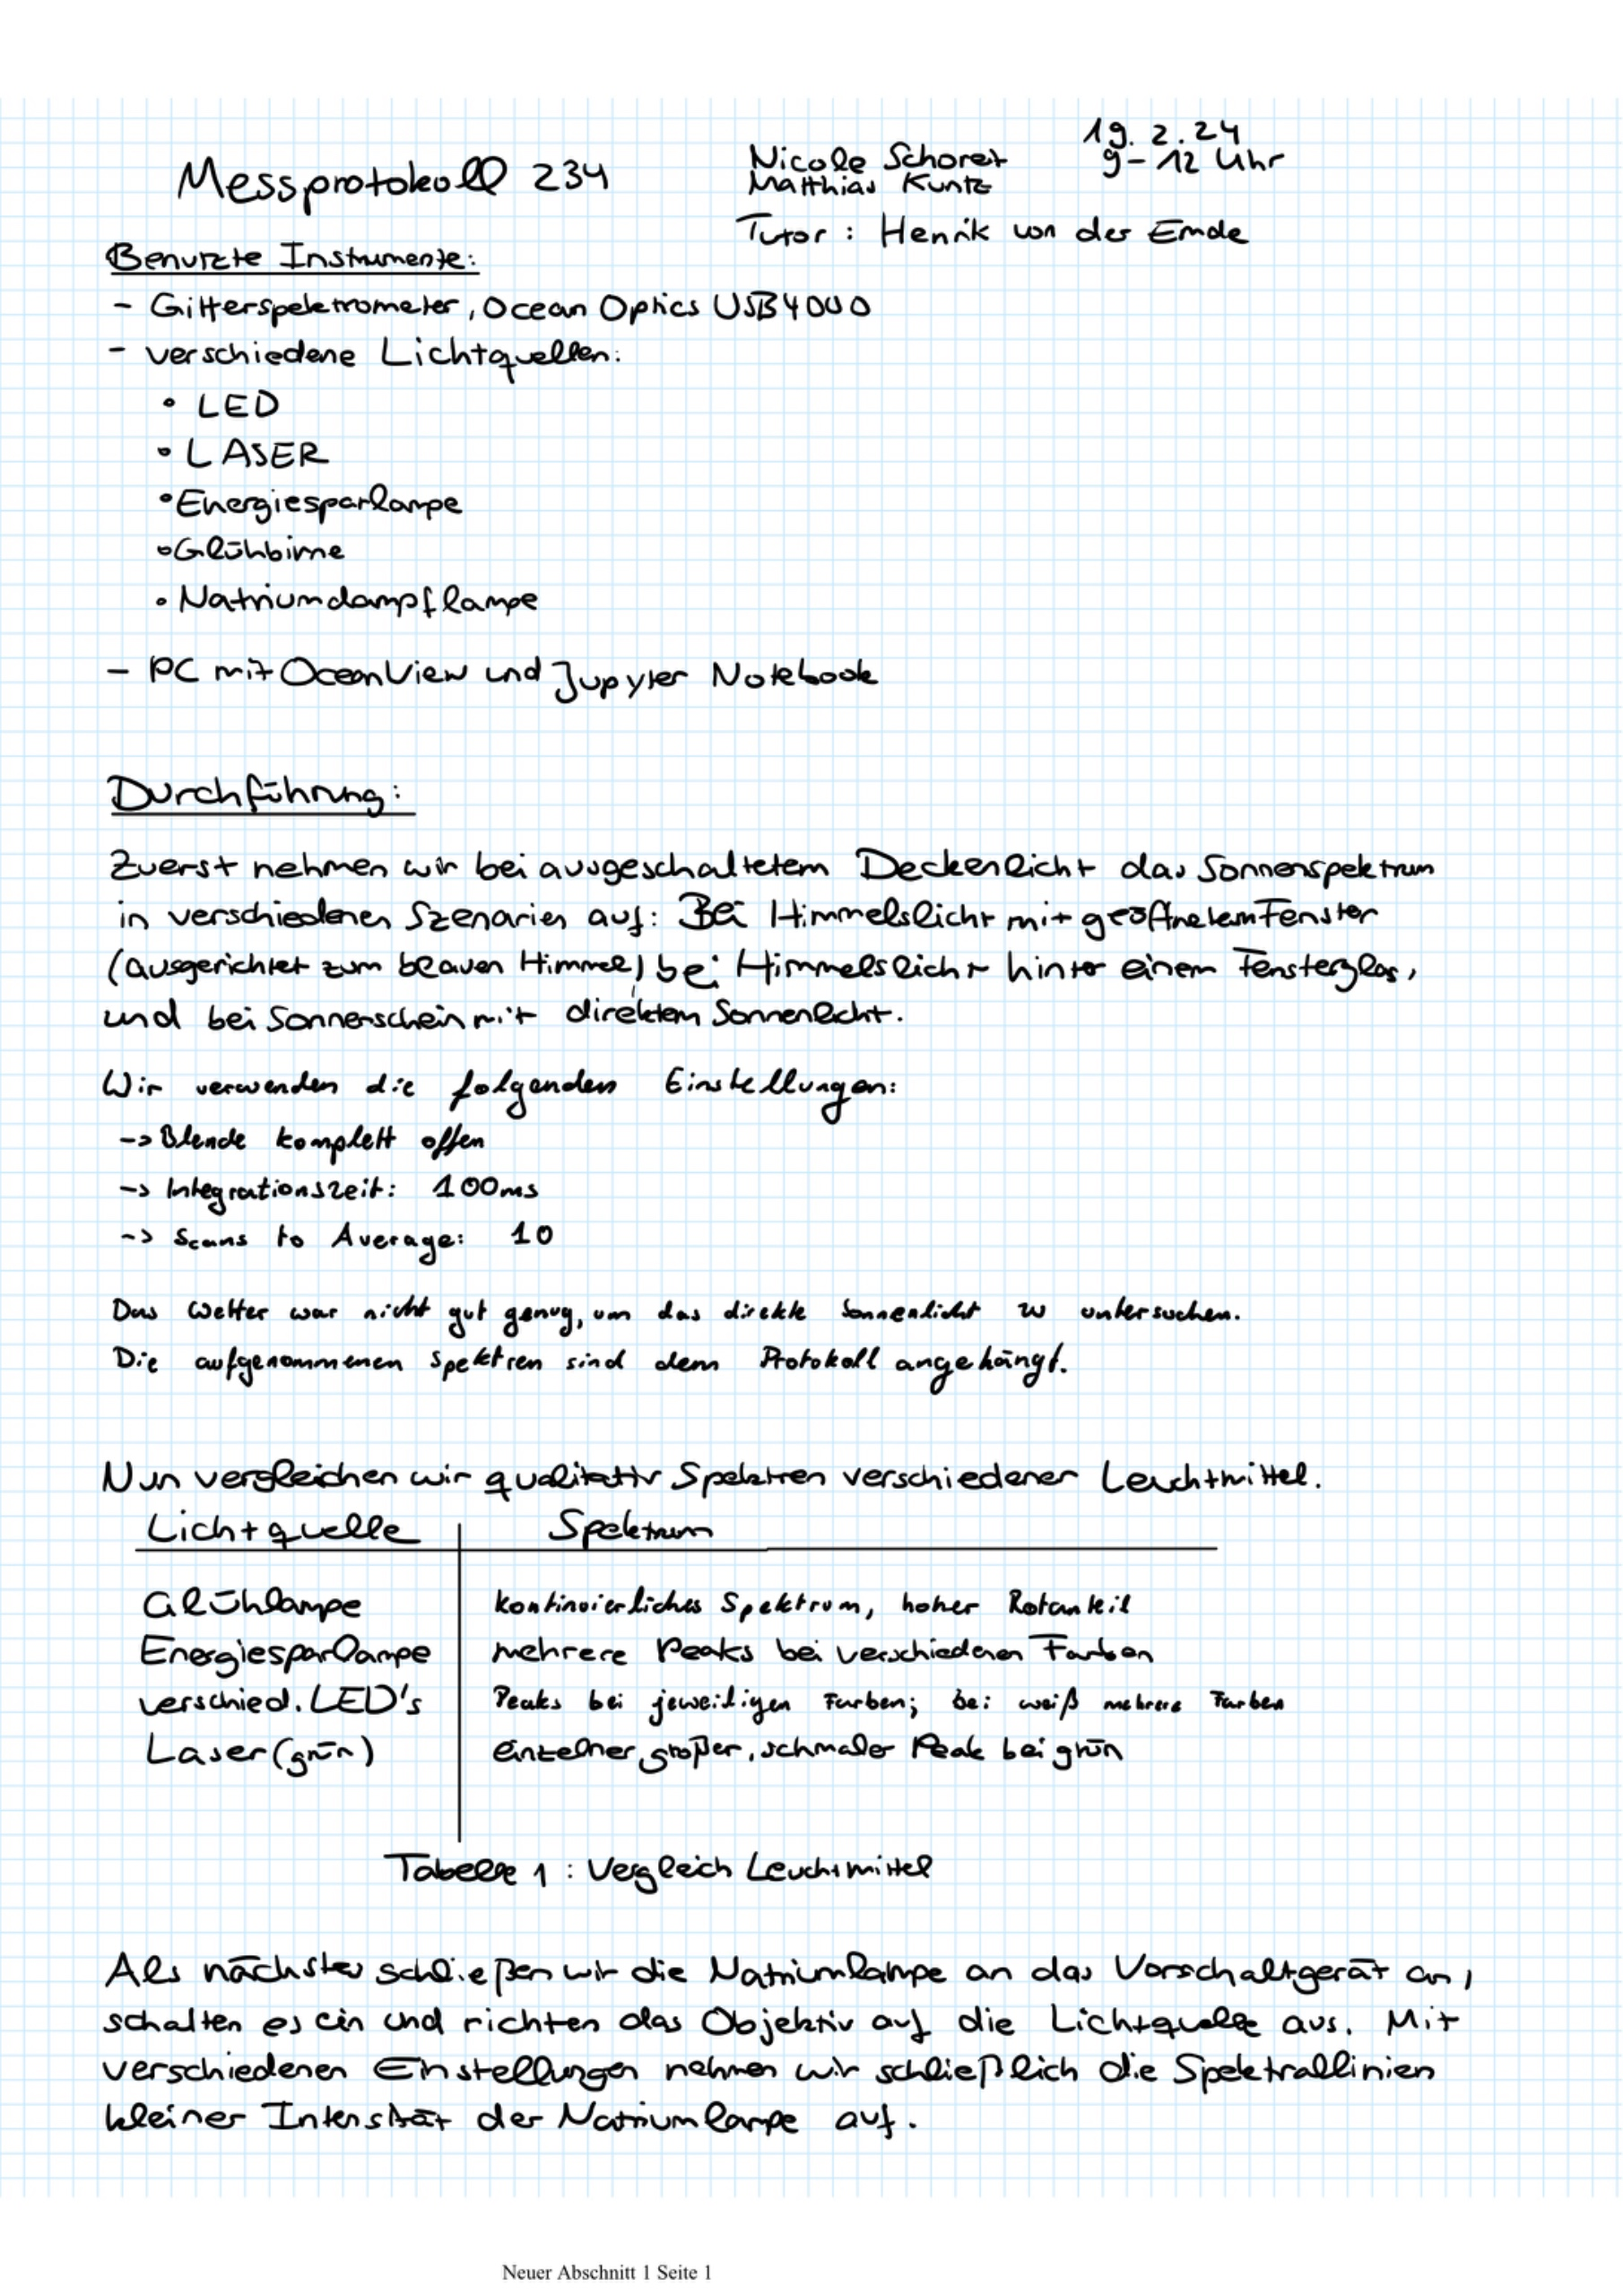
\includegraphics[width=\textwidth]{graphics/mess1.jpeg}
\newpage
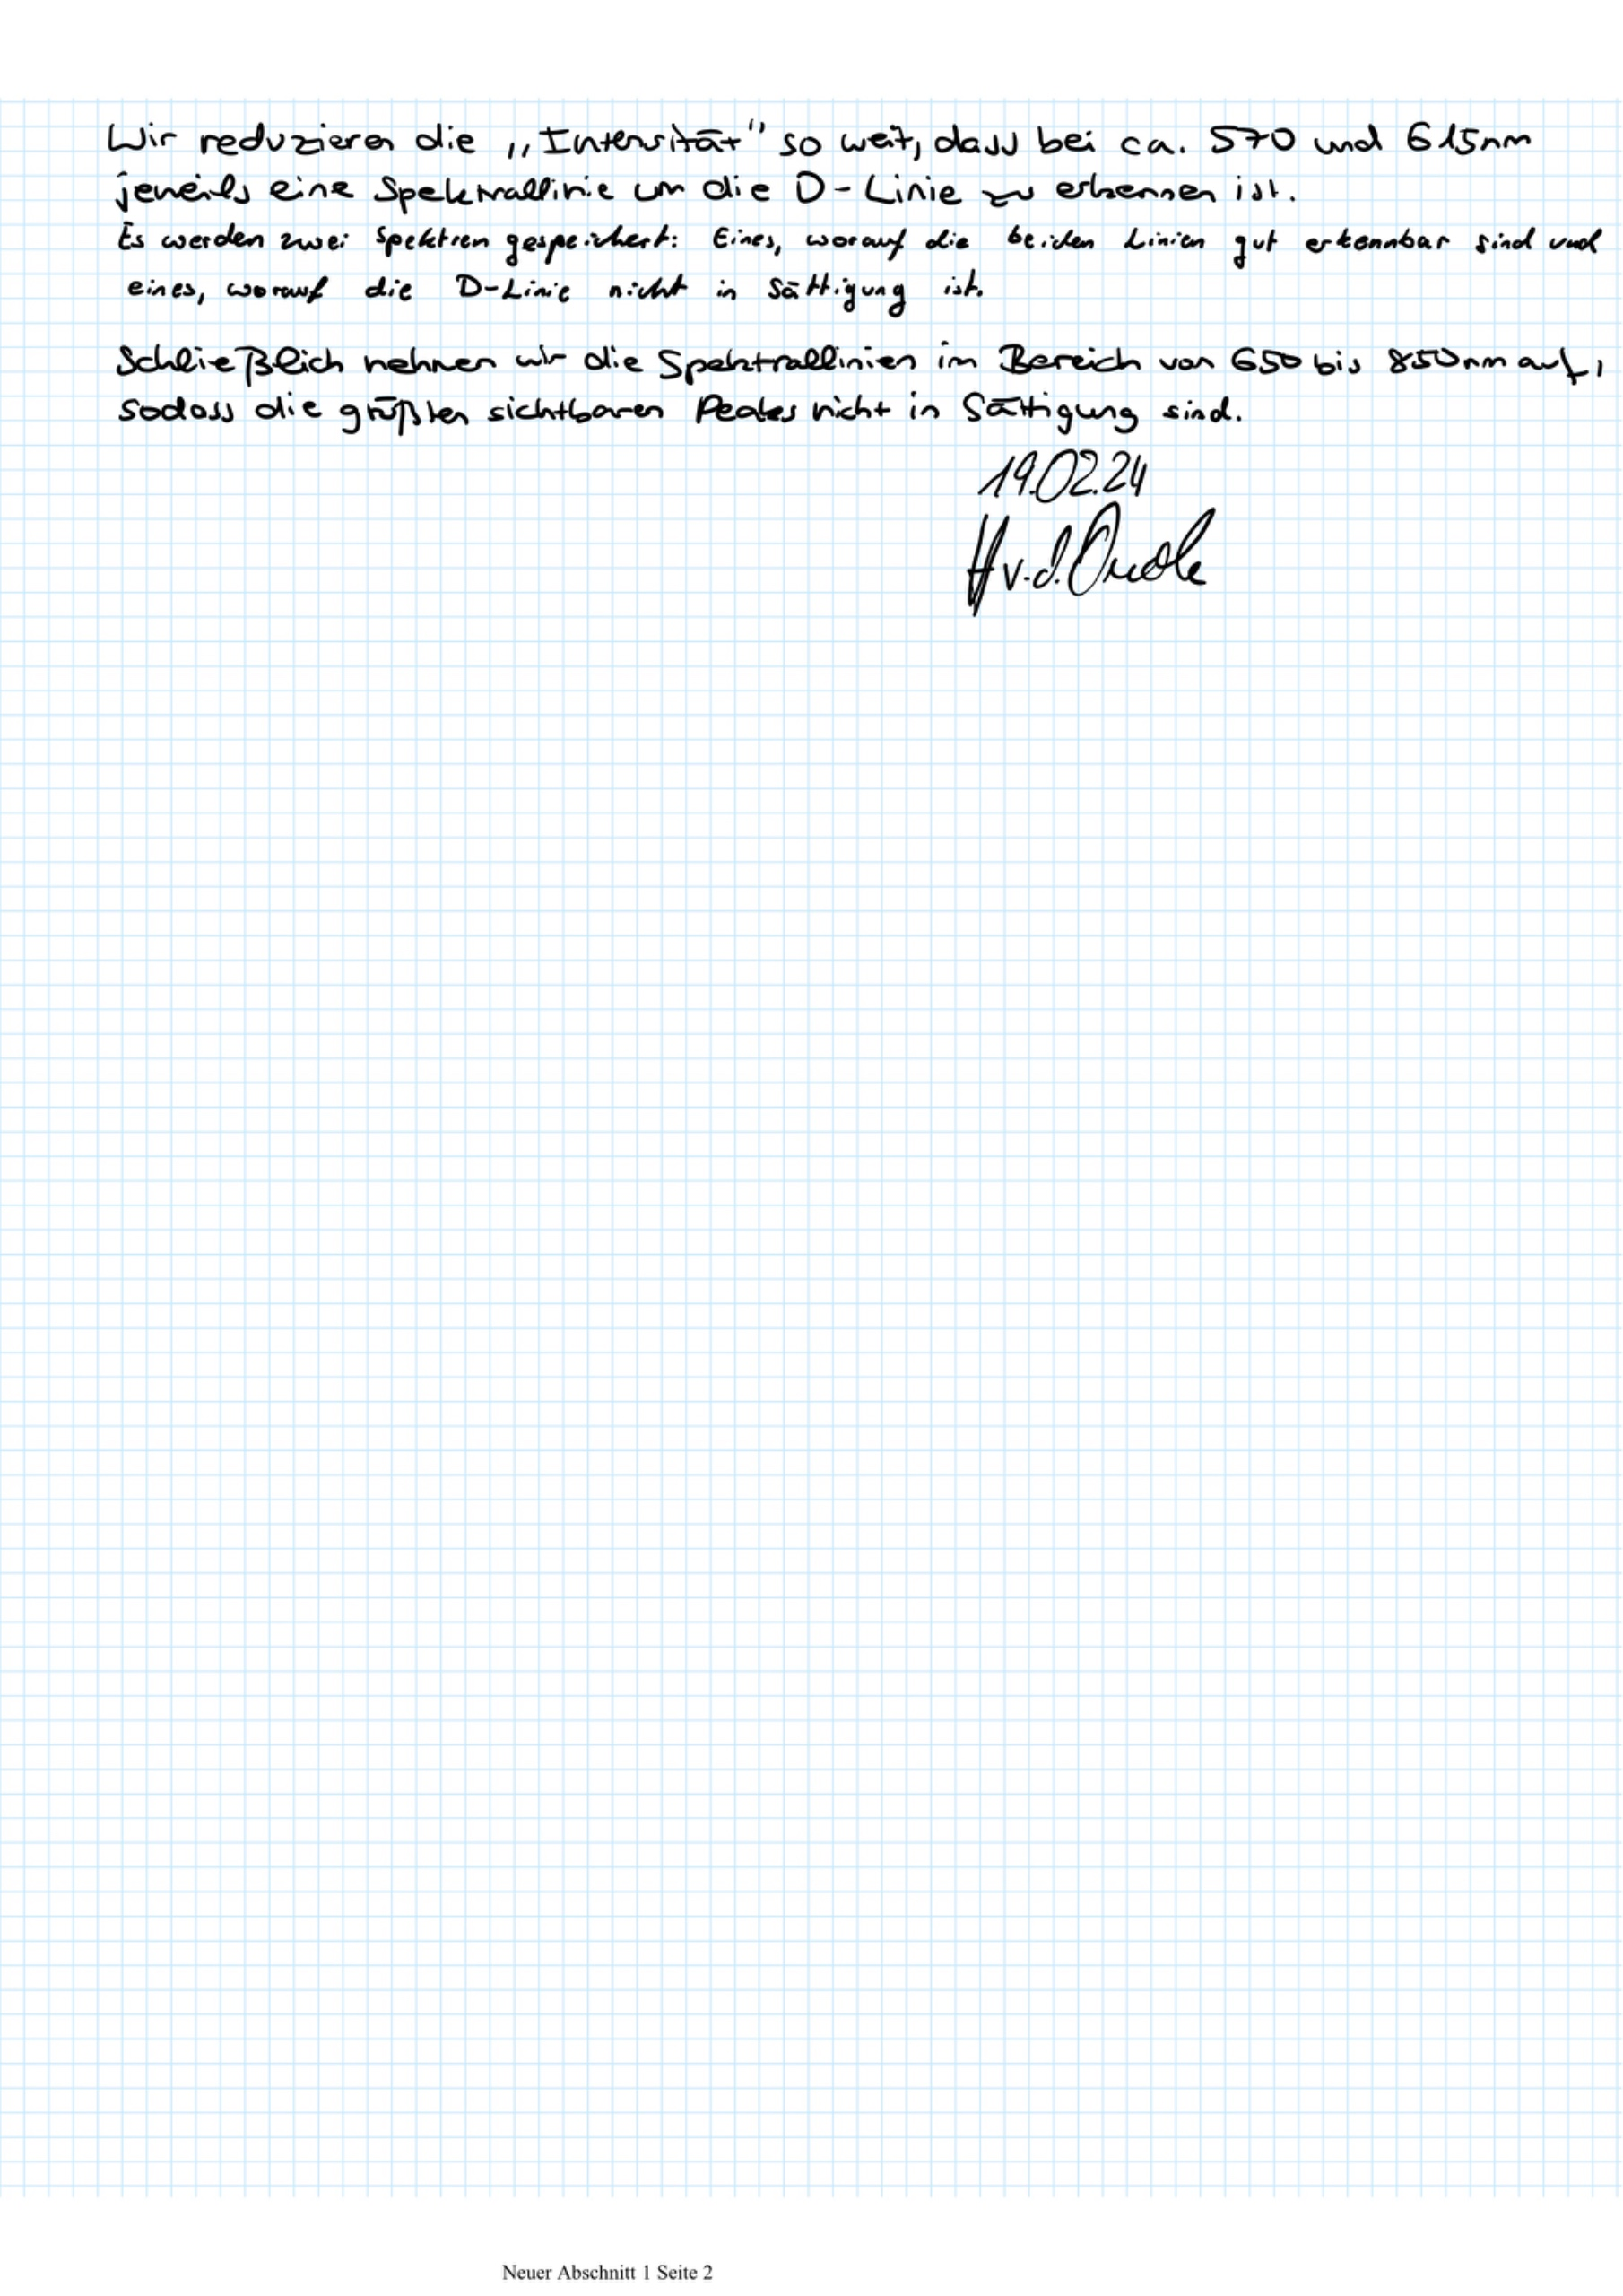
\includegraphics[width=\textwidth]{graphics/mess2.jpeg}
\newpage

\addtocounter{table}{3}

\newpage
%-------------------------AUSWERTUNG-------------------------
\section{Auswertung}

In dieser Evaluation werden alle Fehler, sofern keine spezifische Angabe gemacht wird, mithilfe der Gauss'schen Fehlerfortpflanzung berechnet. Dies bedeutet, dass ein Wert $F$, der mit der Formel $f(a_1, ..., a_n)$ berechnet wird, den Fehler $\Delta F$ annimmt:

\begin{equation}
    \Delta F = \sqrt{\sum_n \left( \frac{\partial f}{\partial a_n} \cdot \Delta a_n \right)^2}.
\end{equation}

Des Weiteren erfolgen Signifikanztests von zwei Werten $a$ und $a'$ über die folgende Formel:

\begin{equation}
    \sigma = \frac{|a-a'|}{\sqrt{(\Delta a)^2 + (\Delta a')^2}}.
\end{equation}

Die Güte eines Fits wird mit der $\chi^2$-Summe bewertet:

\begin{equation}
    \chi^2 = \sum_i^N \left( \frac{\textit{Funktionswert}_i - \textit{Messwert}_i}{\textit{Fehler}_i} \right)^2
\end{equation}

Auch verwendet wird $\chi^2_{red} = \chi^2 / f$, wobei der Freiheitsgrad $f$ die Anzahl der Messwerte minus die Anzahl der Fitparameter ist. Der auf die Freiheitsgrade normierte Wert soll bei einem guten Fit ungefähr 1 sein.

Die Auswertung sowie Berechnung erfolgen über das dem Dokument angehängte Python-Programm.

\newpage

\subsection{Auswertung des Himmelhintergrunds mit und ohne Glas}

\begin{equation}
    \begin{split}
        \Delta \overline{d}_{NaCl} &= \sqrt{\sigma_{std}^2 + \left( \frac{1}{N} \sum_{i=1}^N \Delta d_i \right)^2} \\
        \text{mit} \ \ \ \sigma_{std} &= \sqrt{\frac{1}{N(N-1)} \sum_{i=1}^N (\overline{d} - d_i)^2}.
    \end{split}
\end{equation}


\begin{figure}[h]
  \centering
  \subfloat[Bereich 400-540nm]{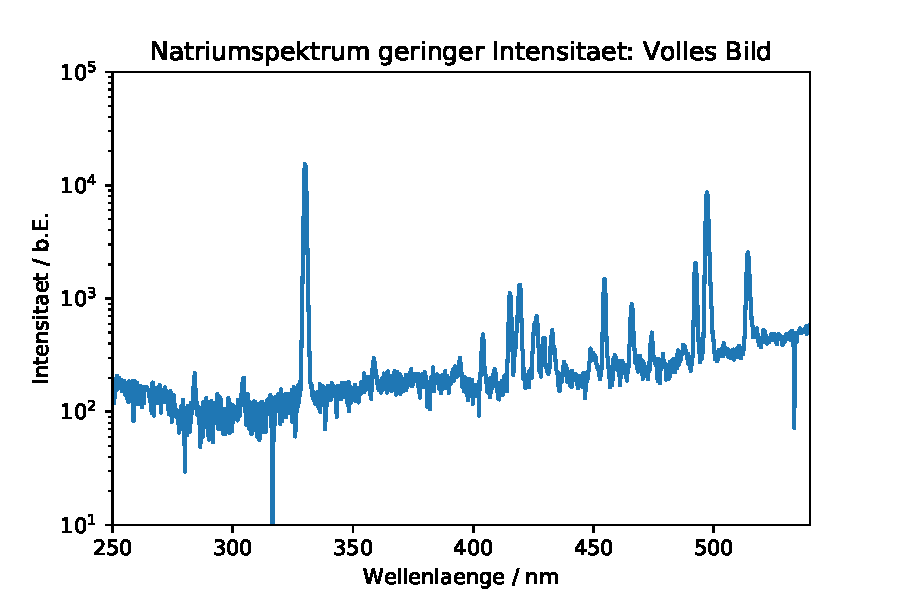
\includegraphics[width=0.48\textwidth]{graphics/outputs/NA_low_full.pdf}\label{fig:NA_low}}
  \hfill
  \subfloat[Bereich 650-800nm]{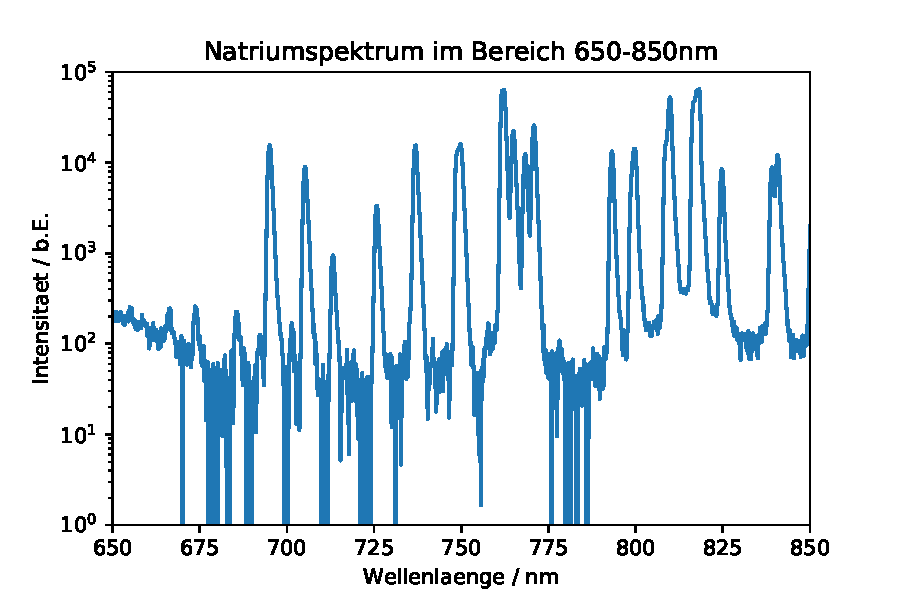
\includegraphics[width=0.48\textwidth]{graphics/outputs/NA_high.pdf}\label{fig:NA_high}}
  \hfill
  \subfloat[D-Linie - Volles Bild]{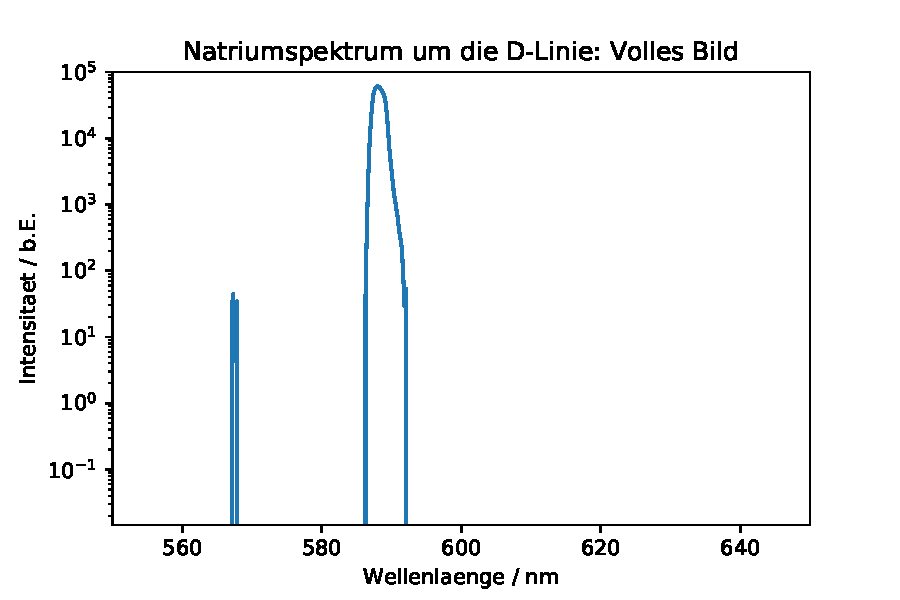
\includegraphics[width=0.48\textwidth]{graphics/outputs/NA_D_full.pdf}\label{fig:NA_D_full}}
  \hfill
  \subfloat[D-Linie - Zoom]{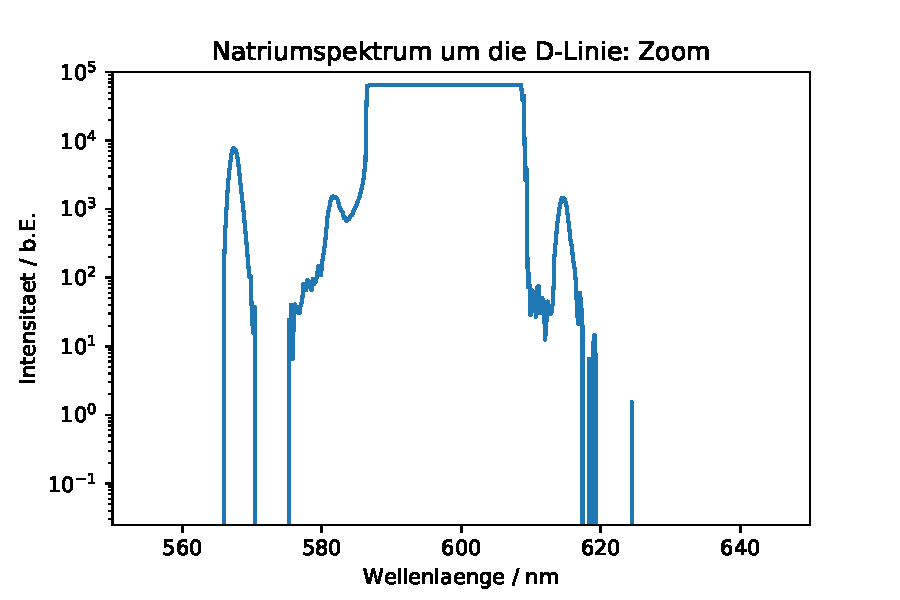
\includegraphics[width=0.48\textwidth]{graphics/outputs/NA_D_zoom.pdf}\label{fig:NA_D_zoom}}
  \hfill
  \caption{Gemessene Spektren der Natriumlampe}
  \label{fig:alleNatriumspektren}
\end{figure}

\phantom{.}

\begin{table}[!h]
    \centering
    %\resizebox{\textwidth}{!}{
    \begin{tabular}{cccc}
        \hline
        \textbf{Kugel} & $\bm{v_{lam}}$ [mm/s] & $\bm{v/v_{lam}}$ & $\bm{Re}$  \\ \hline
        1 & $0,56 \pm 0,06$ & $1,21 \pm 0,18$ & $0,0033 \pm 0,0004$     \\
        2 & $2,23 \pm 0,22$ & $0,95 \pm 0,15$ & $0,0209 \pm 0,0029$     \\
        3 & $5,0 \pm 0,5$   & $0,98 \pm 0,14$ & $0,073 \pm 0,009$     \\
        4 & $8,9 \pm 0,9$   & $0,87 \pm 0,10$ & $0,154 \pm 0,014$     \\
        5 & $13,9 \pm 1,3$  & $0,94 \pm 0,11$ & $0,32 \pm 0,03$     \\
        6 & $20,1 \pm 1,9$  & $0,82 \pm 0,08$ & $0,48 \pm 0,04$     \\
        7 & $27,3 \pm 2,6$  & $0,82 \pm 0,09$ & $0,77 \pm 0,06$     \\
        8 & $36 \pm 3$      & $0,77 \pm 0,08$ & $1,08 \pm 0,09$     \\
        9 & $45 \pm 4$      & $0,74 \pm 0,08$ & $1,48 \pm 0,12$     \\ \hline
    \end{tabular}%}
    \caption{Verhältnis der Geschwindigkeiten \& Reynoldszahlen}
    \label{tab:v_lam&Re}
\end{table}

\phantom{.}

\begin{figure}[!h]
    \centering
    \resizebox{0.9\textwidth}{!}{
    \includegraphics{graphics/outputs/Leuchtkörper-2.pdf}}
    \caption{Vergleich der sechs Leuchtkörper}
    \label{fig:VglLeuchtkörper}
\end{figure}


\newpage
%---------------PRÄSENTATION DER ENDERGEBNISSE---------------
\section{Zusammenfassung der Endergebnisse}

blabla

\newpage
%---------------ZUSAMMENFASSUNG UND DISKUSSION---------------
\section{Diskussion}

blabla

\newpage
%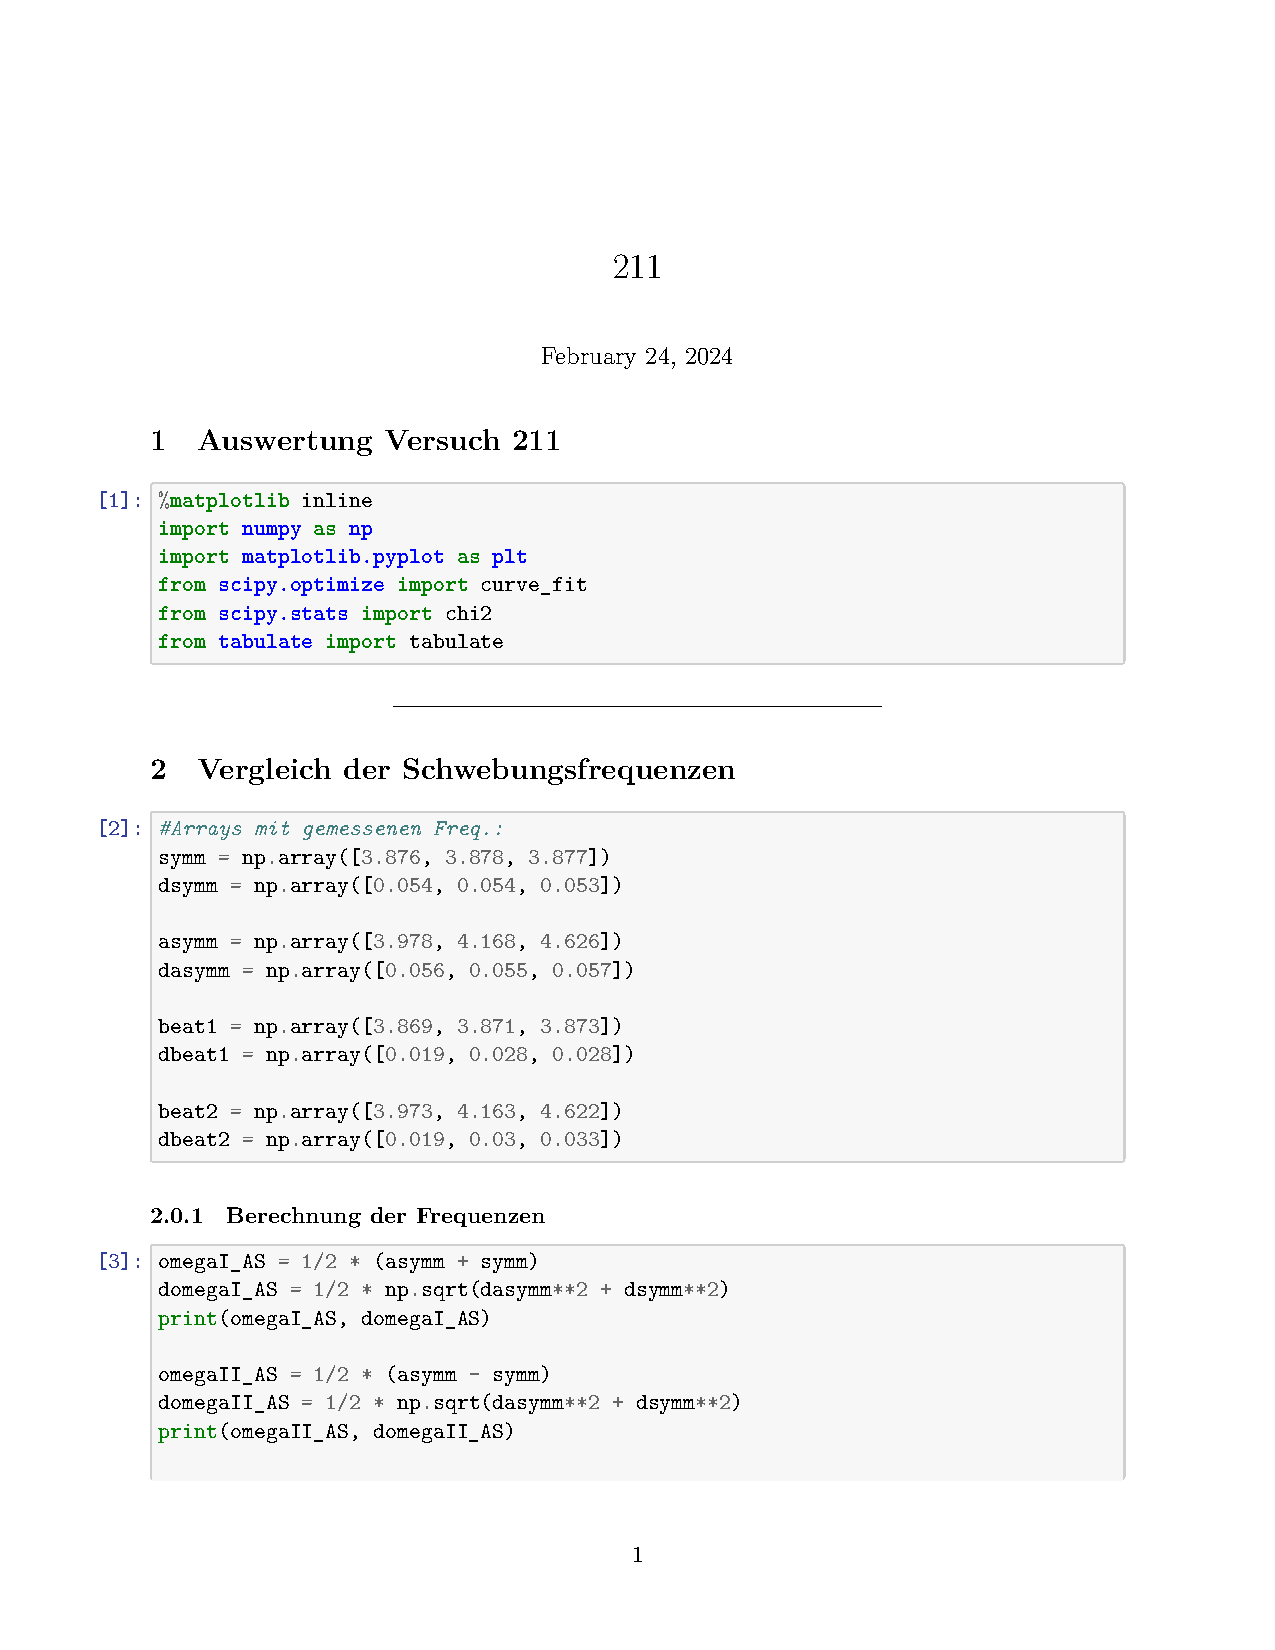
\includepdf[pages=-]{211-1.pdf}

\end{document}

